\documentclass{standalone}
\makeatletter\AtBeginDocument{\@buildstepset{1,2,3}}\makeatother
\usepackage{tikz}
\usetikzlibrary{intersections, calc}
\usepackage{hsbcommon}
    \begin{document}
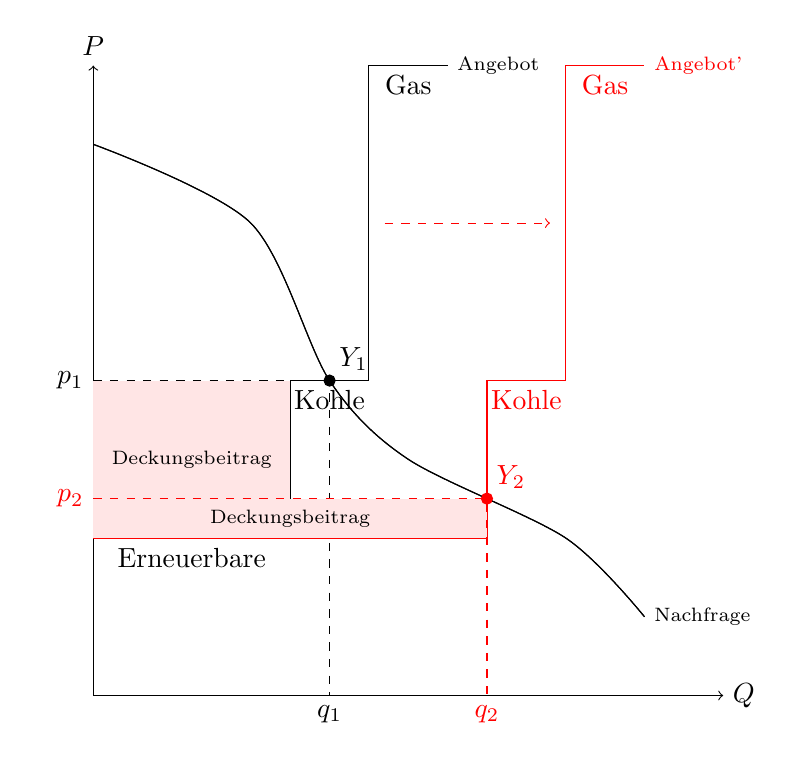
\begin{tikzpicture}
        \draw[->] (0,0) node[below] {\phantom{$X_i$}} -- (8,0) node[right] (Q) {$Q$};
        \draw[->] (0,0) node[left] {\phantom{$Y_mi$}} -- (0,8) node[above] (P) {$P$};


    % Demand curve -- always on
    
        \begin{scope}[color=black]
       
            \coordinate (A) at (0,7);
            \coordinate (B) at (2,6);
            \coordinate (C) at (3,4);
            \coordinate (D) at (4,3);
            \coordinate (E) at (6,2);
            \coordinate (F) at (7,1);
     
            \node[right] at (F) {\scriptsize Nachfrage};
            \draw [name path global=demand] plot [smooth] coordinates {(A) (B) (C) (D) (E) (F)};

        \end{scope}


    %%% Winter scenario

            \coordinate (G) at (0,2);
            \coordinate (H) at (2.5,2);
            \coordinate (I) at (2.5,4);
            \coordinate (J) at (3.5,4);
            \coordinate (K) at (3.5,8);
            \coordinate (L) at (4.5,8);
            
       \ifstep{1}{
        \begin{scope}[color=black]


            \path (G) -- node[below] {Erneuerbare} (H);
            \path (I) -- node[below] {Kohle} (J);
            \path (K) -- node[below] {Gas} (L);
 
           
            \draw [name path=supply] plot  coordinates {(G) (H) (I) (J) (K) (L)};
            \node[right] at (L) {\scriptsize Angebot};
    

            \path [name intersections={of=demand and supply,by=Y}];
            
            \filldraw (Y) circle (2pt) node[above right] {$Y_1$};
            \draw[dashed] (0, |- Y) node[left] {$p_1$} -- (Y) -- (Y |-,0) node[below] {$q_1$};
            
            \draw [name path global=demand] plot [smooth] coordinates {(A) (B) (C) (D) (E) (F)};
            % \filldraw (Y) circle (2pt) node[above right] {\textit{Y}};
            
    
            % \filldraw (I) circle (2pt) node[above right] {\textit{Y}};
    
            
        \end{scope}
}

\ifstep{2}{
            \fill [fill=red!10] (G) rectangle node[black] {\scriptsize Deckungsbeitrag} (I);

}

        \ifstep{3}{
        \begin{scope}[color=red]

            \coordinate (G) at (0,2);
            \coordinate (H) at (5,2);
            \coordinate (I) at (5,4);
            \coordinate (J) at (6,4);
            \coordinate (K) at (6,8);
            \coordinate (L) at (7,8);
    
            \draw[->,dashed,shorten >=0.2cm,shorten <=0.2cm] (3.5,6) -- (6,6);
            
            \draw [name path global=supply] plot  coordinates {(G) (H) (I) (J) (K) (L)};
            \path [name intersections={of=demand and supply,by=Y}];
            \fill [fill=red!10] (G) rectangle node[black] {\scriptsize Deckungsbeitrag} (Y);
            \filldraw (Y) circle (2pt) node[above right] {$Y_2$};
            \node[right] at (L) {\scriptsize Angebot'};
            \draw[dashed] (0, |- Y) node[left] {$p_2$} -- (Y) -- (Y |-,0) node[below] {$q_2$};
    
            \path (I) -- node[below] {Kohle} (J);
            \path (K) -- node[below] {Gas} (L);

        \end{scope}
}

 

        
        
    \end{tikzpicture}
\end{document}
